\documentclass[../main.tex]{subfiles}
\begin{document}

\section{实时搜索、增量式搜索与知识驱动搜索}\label{sec:realtime-incremental-knowledge-search}

\subsection{实时搜索与增量式搜索}\label{sec:realtime-incremental-search}
\begin{enumerate}
    \item \textbf{时间约束下决策：}在有限时间内做出搜索与决策：
        \begin{enumerate}
            \item 需要牺牲最优性来获得可行解
            \item 一次搜索无法遍历完整状态空间
            \item 引入增量式更新与实时反馈机制
        \end{enumerate}
    \item \textbf{实时搜索}
    
    \textcolor{red}{以下内容ppt明显是ai生成，大量不知道从哪拼凑的三点，看一眼得了，反而例题、表格等更有价值；所以对于下面很多概念我都没有做注解，我觉得没有必要浪费我的时间去解读AI产出的史，读者也没有必要花费自己的时间来理解没有经过人类思考而1s内产出的文字。}
    
    \begin{itemize}
        \item \textbf{核心概念：}
        \begin{itemize}
            \item 即时索引
            \item 低延时响应
            \item 持续更新
        \end{itemize}
        \item \textbf{挑战：}
        \begin{itemize}
            \item 数据一致性
            \item 系统性能
            \item 资源消耗
        \end{itemize}
        \item \textbf{数据结构优化：}
        \begin{itemize}
            \item \textbf{倒排索引：}存储从词语到文档的映射，是全文搜索的核心。
            \item \textbf{布隆过滤器：}一种空间效率高的概率数据结构，用于快速判断一个元素是否存在，减少不必要的磁盘查找，但有小概率误判。\textbf{仅会产生 假阳性（误报存在），不会漏掉已存在元素（无假阴性）}
            \item \textbf{LSM树：}优化写密集型场景的持久化存储结构，通过批量写入和后台合并，显著提高写入吞吐量，随机读延迟高于B*树
        \end{itemize}
        \begin{figure}[H]
            \centering
            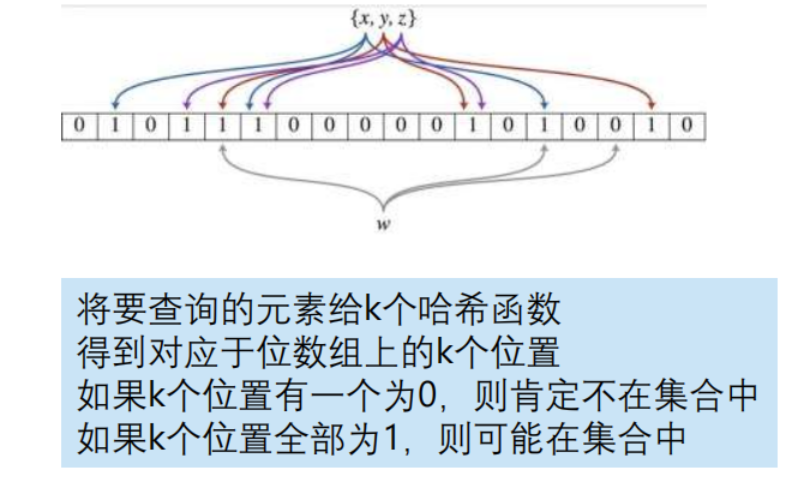
\includegraphics[width=0.5\linewidth]{images/bulong.png}
            \caption{布隆过滤器}
            \label{fig:placeholder}
        \end{figure}
        \item \textbf{关键索引技术：}追求 $O(\log n)$ 甚至 $O(1)$ 的查询开销。
        \begin{itemize}
            \item B+树
            \item 哈希索引
            \item 位图索引
        \end{itemize}
    \end{itemize}
    {\small\kaishu
    \textbf{例：哈希索引}
    
    设哈希函数为
    $$
    h(x)=x\bmod 7
    $$
    对数据元素 $2,6,9,25,63,25,99$ 分别计算哈希值，可得
    $$
    h(2)=2,\quad h(6)=6,\quad h(9)=2,\quad h(25)=4,\quad h(63)=0,\quad h(25)=4,\quad h(99)=1
    $$
    因此，这些数据会按照哈希值被分配到对应的槽中。  
    例如，元素 $2$ 和 $9$ 的哈希值都为 $2$，元素 $25$ 的哈希值为 $4$，说明它们会被映射到同一个槽或桶中。  
    哈希索引的作用，就是先通过哈希函数快速确定数据大致所在的位置，再在对应槽中查找目标元素。  
    它适合处理精确匹配查询，但若多个元素映射到同一位置，就会发生\textbf{冲突}，需要再用链地址法、开放定址法等方式解决。
    
    \bigskip
    
    \textbf{例：位图索引}
    
    现有一张表，共 $8$ 行，包含“性别”和“等级”两列。  
    性别列依次为
    $$
    M,\ F,\ M,\ M,\ F,\ F,\ M,\ F
    $$
    等级列依次为
    $$
    1,\ 2,\ 2,\ 1,\ 3,\ 2,\ 3,\ 1
    $$
    
    为“性别”列建立位图索引：
    
    值 $M$ 的位图为
    $$
    10110010
    $$
    因为第 $1,3,4,7$ 行的性别为 $M$。
    
    值 $F$ 的位图为
    $$
    01001101
    $$
    因为第 $2,5,6,8$ 行的性别为 $F$。
    
    再为“等级”列建立位图索引：
    
    等级 $1$ 的位图为
    $$
    10010001
    $$
    因为第 $1,4,8$ 行的等级为 $1$；
    
    等级 $2$ 的位图为
    $$
    01100100
    $$
    因为第 $2,3,6$ 行的等级为 $2$；
    
    等级 $3$ 的位图为
    $$
    00001010
    $$
    因为第 $5,7$ 行的等级为 $3$。
    
    若查询“\textbf{性别为 $M$ 且等级为 $2$ 的员工}”，只需取出对应位图
    $$
    10110010
    $$
    和
    $$
    01100100
    $$
    然后做按位与运算：
    $$
    10110010 \land 01100100 = 00100000
    $$
    结果中只有第 $3$ 位为 $1$，因此满足条件的是\textbf{第 $3$ 行}。
    
    位图索引的本质，是把“某一行是否满足某个取值条件”编码成 $0/1$，这样多个条件查询就可以直接转化为位运算。  
    它特别适合像性别、等级这种\textbf{取值种类少}的属性。
    }
    \item \textbf{RTA*（Real-Time A*）}
    \begin{itemize}
        \item \textbf{基本思想：}每次仅探索有限深度；根据启发值选择下一步，并更新已访问状态的代价；适合动态、时间受限的环境
        
        \item \textbf{评价方式：}在当前状态 $s$ 下，对每个可行动作 $a\in \mathrm{Actions}(s)$，计算
        $$
        Q(a)=\mathrm{StepCost}\bigl(s,a,\mathrm{Result}(s,a)\bigr)+h\bigl(\mathrm{Result}(s,a)\bigr)
        $$
        即“走这一步的实际代价 $+$ 后继状态的启发式估计”。
        
        \item \textbf{动作选择：}选择使 $Q(a)$ 最小的动作 $a^*$，执行后将当前状态更新为
        $$
        s\leftarrow \mathrm{Result}(s,a^*)
        $$
        
        \item \textbf{学习/更新：}在做出一步动作后，可根据本次局部搜索结果更新当前状态或已访问状态的启发值，使以后再次到达这些状态时有更准确的估计。
        
        \item \textbf{时间复杂度：}单步决策通常为
        $$
        O(b^L)
        $$
        其中 $b$ 为分支因子，$L$ 为每一步允许的前瞻深度；

        \item \textbf{空间复杂度：}通常为
        $$
        O\!\left(|V_{\mathrm{visited}}|+b^L\right)
        $$
        其中 $|V_{\mathrm{visited}}|$ 表示已访问状态中被记录启发值的状态数；若只看单步前瞻部分，可近似记为
        $$
        O(b^L)
        $$
        因而显著低于需要维护全局 frontier 的 A*。
        
        \item \textbf{适用场景：}动态环境、时间受限环境，或无法承担 A* 大规模存储开销的场景。
        
        \item \textbf{算法变种：}
        \begin{itemize}
            \item \textbf{LRTA*（Learning Real-Time A*）：}在每次移动后更新已访问状态的启发值，即加入“学习”机制；
            \item \textbf{RTAA*（Real-Time Adaptive A*）：}在 RTA* 基础上加入有限深度前瞻搜索，即一次看得更远；
            \item \textbf{DTA*（Dynamic Real-Time A*）：}面向动态环境进一步调整搜索与更新策略，即增强对环境变化的适应性。
        \end{itemize}
    \end{itemize}
    \item \textbf{IDS（Iterative Deepening Search，迭代加深搜索）}
    \begin{itemize}
        \item \textbf{要点：}在深度受限搜索的基础上逐步增加深度上限，兼顾 DFS 的空间优势与 BFS 的浅层优先特性；
        \item \textbf{解释：}从深度上限 $0$ 开始，每轮执行一次深度受限 DFS；若当前深度找到目标则立即返回，否则继续增大深度上限重新搜索；
        \item \textbf{时间复杂度：}
        $$
        O(b^d)
        $$
        \item \textbf{空间复杂度：}
        $$
        O(bd)
        $$
        \item \textbf{算法变种：}
        \begin{itemize}
            \item \textbf{IDDFS（Iterative Deepening Depth-First Search）：}每轮把深度上限加 $1$，即标准的迭代加深 DFS\textcolor{red}{做PPT的时候看到这个不想笑吗，自己是自己的变种}；
            \item \textbf{IDA*（Iterative Deepening A*）：}把“深度上限”改为“$f$ 代价上限”，即用代价阈值替代层数阈值；
        \end{itemize}
    \end{itemize}
    \item \textbf{动态规划与求解}
    \begin{itemize}
        \item \textbf{增量式搜索：}复用先前的计算结果来加速新解的生成\footnote{避免每次从头开始计算，而是通过复用前一个实例的中间结果或数据结构，仅对问题发生变化的局部进行更新。}，核心特点是：
        \begin{itemize}
            \item 结果复用
            \item 局部更新
            \item 动态适应
        \end{itemize}
        \item \textbf{增量式求解：}\textcolor{red}{懒得喷，在这车轱辘话，就是增量式搜索，搜索就是求解啊}
        \item \textbf{动态规划（DP）：}把多阶段问题变换为一系列相互联系的的单阶段问题，然后逐个加以
解决，各个阶段决策的选取仅依赖当前状态（马尔可夫性），适用问题满足：
        \begin{itemize}
            \item \textbf{最优子结构：}整体最优由子问题最优构成
            \item \textbf{重叠子问题：}子问题被重复求解，缓存可复用
        \end{itemize}
        经典例子包括：背包问题、最短路径、最长公共子序列(LCS)等；
    \end{itemize}
    \item \textbf{D* Lite}
    \begin{itemize}
        \item \textbf{定位：}将\textbf{动态规划}与\textbf{增量式求解}结合起来的重规划算法；
        \textcolor{red}{注意这里的$g$与前面的不同，这里指的是$h$；$rhs$是每个节点经过遍历以后，已经记录下来的到终点的c+g（即原来的g+h）；所以增量式在哪里呢？就是如果发现某个边被变化了，到对应的被变化的节点，去算一下这个节点新的rhs，和固定的用来预测的g对比一下，如果rhs比g小，说明有新的路径更优，那么g估计的就不准了，把g更新为rhs；如果rhs比g大，那说明g估计的太乐观了，要重新把g设置为无穷来重新估计}
        \item \textbf{核心量：}
        \begin{itemize}
            \item $g(s)$：当前从节点 $s$ 到目标的实际最短路径代价的当前最佳估计\footnote{注意这里与之前的$g$不一样，更像是$h$}；
            \item $rhs(s)$：一步前瞻值\footnote{说人话就是走这一步的代价，什么前瞻值，也不知道哪里翻译来的}，由后继节点的 $g$ 值计算得到，
            $$
            rhs(s)=\min_{s'\in Succ(s)}\bigl(c(s,s')+g(s')\bigr)
            $$
            它表示根据当前已知信息，从 $s$ 出发可达到的最优代价；
            \item 若 $g(s)=rhs(s)$，则称节点 $s$ \textbf{一致}；否则称为\textbf{不一致}，需要更新；
            \item 优先级由
            $$
            key(s)=\Bigl[\min(g(s),rhs(s))+h(s,s_{start}),\ \min(g(s),rhs(s))\Bigr]
            $$
            决定。
        \end{itemize}
        {\small\kaishu
        \item \textbf{$rhs$ 的直观理解：}  
        $rhs(s)$ 可以理解为节点 $s$ 的“一步前瞻最优值”，即：根据当前各个后继节点已经记录的 $g$ 值，反推出从 $s$ 出发到目标的当前最优代价估计：
        $$
        rhs(s)=\min_{s'\in Succ(s)}\bigl(c(s,s')+g(s')\bigr)
        $$
        其中，$Succ(s)$ 表示 $s$ 的后继节点集合，$c(s,s')$ 表示从 $s$ 到 $s'$ 的边代价。
        
        {\small\kaishu
        例如，设节点 $s$ 有两个后继节点 $a,b$，并且
        $$
        c(s,a)=2,\qquad g(a)=5
        $$
        $$
        c(s,b)=3,\qquad g(b)=10
        $$
        则
        $$
        rhs(s)=\min\{c(s,a)+g(a),\ c(s,b)+g(b)\}
        $$
        $$
        =\min\{2+5,\ 3+10\}
        =\min\{7,\ 13\}
        =7
        $$
        这说明：按照当前已知信息，从节点 $s$ 出发到目标的最优走法，是先走到 $a$，总代价估计为 $7$。
        
        若此时节点 $s$ 当前记录的值为
        $$
        g(s)=9
        $$
        则说明当前记录偏大，因为
        $$
        g(s)>rhs(s)
        $$
        表示已经找到了一条更优路径，应将 $g(s)$ 向 $rhs(s)$ 修正。
        
        若
        $$
        g(s)=7
        $$
        则有
        $$
        g(s)=rhs(s)
        $$
        说明该节点当前是一致的。
        
        若
        $$
        g(s)=4
        $$
        则有
        $$
        g(s)<rhs(s)
        $$
        说明当前记录过于乐观，已经不能由当前后继信息支持，需要重新增大并继续传播更新。
        }
                
        
        }
        \item \textbf{执行过程：}
        \begin{itemize}
            \item \textbf{初始化：}所有节点 $g=\infty,\ rhs=\infty$，令目标节点或反向搜索起点的 $rhs=0$，并按 $key$ 入优先队列；
            \item \textbf{主循环：}每次弹出最小 $key$ 的节点；若 $g(s)>rhs(s)$，则说明找到了更优路径，令 $g(s)\leftarrow rhs(s)$；若 $g(s)<rhs(s)$，则说明旧估计偏小，令 $g(s)\leftarrow \infty$ 后重新计算，并把受影响前驱继续更新；
            \item \textbf{动态更新：}边代价变化时，只局部刷新相关节点的 $rhs$ 并重新入队，再运行主循环即可快速重规划；
            \item \textbf{路径输出：}从当前节点出发，沿着使 $c(s,s')+g(s')$ 最小的后继前进，直到到达目标或判定不可达。
        \end{itemize}
    \end{itemize}
    
    \item \textbf{Anytime Dynamic A*（AD*）}
    \begin{itemize}
        \item \textbf{定位：}把 D* Lite 的增量式重规划能力与 Anytime Repairing A*（ARA*）的启发式膨胀机制结合起来，用于动态环境中的“速度--解质量”权衡。
        \item \textbf{核心思想：}
        \begin{itemize}
            \item 先使用大于 $1$ 的膨胀因子 $\varepsilon$，快速求得一条次优但有质量保证的路径；
            \item 随着时间增加，逐步减小 $\varepsilon$，持续改进路径质量；
            \item 当环境发生变化时，不从头开始，而是像 D* Lite 一样利用已有结果做增量式修补。
        \end{itemize}
        \item \textbf{关键参数：}
        \begin{itemize}
            \item $\varepsilon$ 是 AD* 的关键参数，表示对启发式函数乐观程度的膨胀因子；
            \item $\varepsilon$ 较大时，搜索更快，但解更粗；
            \item $\varepsilon$ 逐步减小时，解会不断逼近最优解。
        \end{itemize}
        \item \textbf{特点：}
        \begin{itemize}
            \item 能在时间有限时先给出可用解；
            \item 之后可继续优化，逐步提高路径质量；
            \item 比单纯的 D* Lite 更强调 anytime 性，先给答案，再逐步变好；
            \item 适合实时性要求高、环境又可能动态变化的场景。
        \end{itemize}
    \end{itemize}
\end{enumerate}
\begin{center}
\renewcommand{\arraystretch}{1.25}
\begin{tabularx}{\textwidth}{>{\raggedright\arraybackslash}p{2.2cm}
>{\raggedright\arraybackslash}X
>{\raggedright\arraybackslash}X}
\toprule
算法 & 优点 & 缺点 \\
\midrule
RTA* 
& 决策速度快，适合时间约束很紧的场景；即使在未知或部分可知环境中，也能快速给出可行解。
& 通常只能得到次优路径，难以保证最优性；对启发式函数质量依赖较强。 \\

D* Lite
& 适合动态环境中的增量式重规划；能够复用已有计算结果，环境变化后只需局部修补，重新计算开销较小；可找到最优路径。
& 实现比 RTA* 更复杂；当环境变化较大或变化过于频繁时，仍可能需要较多计算才能重新收敛。 \\

AD*
& 结合了 D* Lite 的增量式重规划能力与 Anytime 方法的“先给可用解、再逐步优化”特点；能较快给出有质量保证的次优解，并随着时间推移不断逼近最优。
& 实现最复杂；需要调节启发式膨胀因子 $\varepsilon$，以权衡搜索速度与解的质量。 \\
\bottomrule
\end{tabularx}
\end{center}
\subsection{知识驱动的搜索}\label{sec:knowledge-driven-search}
\begin{enumerate}
    \item \textbf{多阶段决策优化}
    \begin{itemize}
        \item \textbf{定义：}多阶段决策优化框架是把求解过程按时间或步数\textbf{离散为一系列阶段}的建模与求解范式。
        \item \textbf{要点：}
        \begin{itemize}
            \item 状态表示
            \item 阶段转移函数
            \item 优化策略
        \end{itemize}
    \end{itemize}
    \item \textbf{领域知识集成}
    \begin{itemize}
        \item \textbf{领域知识：}领域知识是指与具体问题域固有的先验事实、约束、规律与结构信息的集合
        \item \textbf{如何帮助搜索？}
        \begin{itemize}
            \item 缩小搜索空间（提前排除无效路径）
            \item 改进启发函数的准确性
            \item 引导搜索靠近可行或高价值区域
        \end{itemize}
        \item \textbf{知识表示技术：}规则库、本体论、专家系统
        \item \textbf{知识驱动的搜索优化技术：}剪枝策略、启发式改进、约束传播  
        \item \textbf{知识图谱在搜索中的应用：}实体关系建模、语义搜索、知识推理
        \item \textbf{知识图谱构建技术：}实体抽取、关系抽取、知识融合
    \end{itemize}
    \item \textbf{基于逻辑的搜索}
    \begin{itemize}
        \item \textbf{基本思想：}用逻辑公式表达约束条件与状态关系，在搜索过程中借助逻辑推理进行剪枝，不满足约束的分支可直接排除。
        \item \textbf{典型问题：}SAT 求解、约束满足问题（CSP）。
        
        \textbf{SAT求解：}
            \begin{itemize}
            \item \textbf{SAT 问题：}给定一个布尔公式，判断是否存在一组变量赋值使公式为真。SAT 是第一个被证明为 NP-完全的问题。
            \item \textbf{基本求解框架：}经典 SAT 求解以 DPLL 算法为基础，通过回溯搜索结合剪枝来系统探索解空间。
            \item \textbf{常用推理规则：}
            \begin{itemize}
                \item \textbf{单元归结（unit resolution）：}若子句中只剩一个文字可满足，则可直接推出该文字必须取真，并继续化简其余子句。
                \item \textbf{全归结（full resolution）：}对含互补文字的两个子句做消解，删去这一对互补文字，得到新的子句，用于推出隐含约束。
            \end{itemize}
            \item \textbf{现代 SAT 技术：}在 DPLL 基础上，现代 SAT 求解器进一步引入冲突驱动的子句学习（CDCL）、动态重启策略以及更高效的数据结构，以提高大规模复杂问题的求解效率。
        \end{itemize}

        \textbf{CSP求解：}
        \begin{itemize}
            \item \textbf{CSP：}CSP 由变量、值域、约束三部分组成；常见方法包括回溯搜索与约束传播。
        \end{itemize}
    \end{itemize}

    {\small\kaishu
例1：AC-3 约束传播过程。

设有三个变量
$$
A,\;B,\;C
$$
其值域分别为
$$
D(A)=\{1,2,3\},\qquad D(B)=\{1,2,3\},\qquad D(C)=\{1,2,3\}
$$
约束为
$$
A<B,\qquad B<C,\qquad A\neq C
$$

因此初始弧队列可写为
$$
(A,B),\ (B,A),\ (B,C),\ (C,B),\ (A,C),\ (C,A)
$$

\textbf{第1步：处理 $(A,B)$，约束 $A<B$。}

检查 $A$ 的每个取值：
$$
A=1:\ \exists\,B=2\text{ 或 }3,\ \text{使得 }1<B
$$
$$
A=2:\ \exists\,B=3,\ \text{使得 }2<B
$$
$$
A=3:\ \nexists\,B\in\{1,2,3\}\text{ 使得 }3<B
$$
故删除 $A=3$，得到
$$
D(A)=\{1,2\}
$$
由于 $D(A)$ 被修改，将所有指向 $A$ 的弧（除当前对应反向弧 $(B,A)$ 外）重新加入队列，因此加入
$$
(C,A)
$$
此时队列可记为
$$
(B,A),\ (B,C),\ (C,B),\ (A,C),\ (C,A)
$$

\textbf{第2步：处理 $(B,A)$，约束仍等价于 $A<B$。}

检查 $B$ 的每个取值，此时
$$
D(A)=\{1,2\}
$$
$$
B=1:\ \nexists\,A\in\{1,2\}\text{ 使得 }A<1
$$
$$
B=2:\ \exists\,A=1,\ \text{使得 }A<2
$$
$$
B=3:\ \exists\,A=1\text{ 或 }2,\ \text{使得 }A<3
$$
故删除 $B=1$，得到
$$
D(B)=\{2,3\}
$$
由于 $D(B)$ 被修改，将所有指向 $B$ 的弧（除当前对应反向弧 $(A,B)$ 外）重新加入队列，因此加入
$$
(C,B)
$$
此时队列可记为
$$
(B,C),\ (C,B),\ (A,C),\ (C,A),\ (C,B)
$$

\textbf{第3步：处理 $(B,C)$，约束 $B<C$。}

检查 $B$ 的每个取值，此时
$$
D(B)=\{2,3\},\qquad D(C)=\{1,2,3\}
$$
$$
B=2:\ \exists\,C=3,\ \text{使得 }2<C
$$
$$
B=3:\ \nexists\,C\in\{1,2,3\}\text{ 使得 }3<C
$$
故删除 $B=3$，得到
$$
D(B)=\{2\}
$$
由于 $D(B)$ 再次被修改，将所有指向 $B$ 的弧（除当前对应反向弧 $(C,B)$ 外）重新加入队列，因此加入
$$
(A,B)
$$
此时队列可记为
$$
(C,B),\ (A,C),\ (C,A),\ (C,B),\ (A,B)
$$

\textbf{第4步：处理 $(C,B)$，约束仍等价于 $B<C$。}

检查 $C$ 的每个取值，此时
$$
D(B)=\{2\}
$$
$$
C=1:\ \nexists\,B=2\text{ 使得 }2<1
$$
$$
C=2:\ \nexists\,B=2\text{ 使得 }2<2
$$
$$
C=3:\ \exists\,B=2,\ \text{使得 }2<3
$$
故删除 $C=1,2$，得到
$$
D(C)=\{3\}
$$
由于 $D(C)$ 被修改，将所有指向 $C$ 的弧（除当前对应反向弧 $(B,C)$ 外）重新加入队列，因此加入
$$
(A,C)
$$
此时队列可记为
$$
(A,C),\ (C,A),\ (C,B),\ (A,B),\ (A,C)
$$

\textbf{第5步：处理 $(A,C)$，约束 $A\neq C$。}

此时
$$
D(A)=\{1,2\},\qquad D(C)=\{3\}
$$
检查 $A$ 的每个取值：
$$
A=1:\ \exists\,C=3,\ \text{使得 }1\neq 3
$$
$$
A=2:\ \exists\,C=3,\ \text{使得 }2\neq 3
$$
因此 $D(A)$ 不变，即
$$
D(A)=\{1,2\}
$$
队列不新增弧。

\textbf{第6步：处理 $(C,A)$，约束仍为 $A\neq C$。}

检查 $C$ 的取值：
$$
C=3:\ \exists\,A=1\text{ 或 }2,\ \text{使得 }A\neq 3
$$
因此 $D(C)$ 不变，即
$$
D(C)=\{3\}
$$
队列不新增弧。

\textbf{第7步：处理 $(C,B)$，约束 $B<C$。}

此时
$$
D(B)=\{2\},\qquad D(C)=\{3\}
$$
检查 $C=3$：
$$
\exists\,B=2,\ \text{使得 }2<3
$$
因此 $D(C)$ 不变，队列不新增弧。

\textbf{第8步：处理 $(A,B)$，约束 $A<B$。}

此时
$$
D(A)=\{1,2\},\qquad D(B)=\{2\}
$$
检查 $A$ 的每个取值：
$$
A=1:\ \exists\,B=2,\ \text{使得 }1<2
$$
$$
A=2:\ \nexists\,B=2\text{ 使得 }2<2
$$
故删除 $A=2$，得到
$$
D(A)=\{1\}
$$
由于 $D(A)$ 被修改，将所有指向 $A$ 的弧（除当前对应反向弧 $(B,A)$ 外）重新加入队列，因此加入
$$
(C,A)
$$
此时队列可记为
$$
(A,C),\ (C,A)
$$

\textbf{第9步：处理 $(A,C)$，约束 $A\neq C$。}

此时
$$
D(A)=\{1\},\qquad D(C)=\{3\}
$$
检查 $A=1$：
$$
\exists\,C=3,\ \text{使得 }1\neq 3
$$
因此 $D(A)$ 不变，队列不新增弧。

\textbf{第10步：处理 $(C,A)$，约束 $A\neq C$。}

检查 $C=3$：
$$
\exists\,A=1,\ \text{使得 }1\neq 3
$$
因此 $D(C)$ 不变，队列不新增弧。

至此队列为空，AC-3 结束。最终结果为
$$
D(A)=\{1\},\qquad D(B)=\{2\},\qquad D(C)=\{3\}
$$
}

    \item \textbf{学习与搜索结合}
    \begin{itemize}
        \item \textbf{为什么要结合：}
        \begin{itemize}
            \item 搜索提供全局结构探索，学习提供局部策略优化；
            \item 可以在线调整启发式函数；
            \item 数据驱动可提升搜索效率、鲁棒性与适应性。
        \end{itemize}

        \item \textbf{常见形式：}
        \begin{itemize}
            \item \textbf{强化学习：}通过与环境交互学习搜索策略或价值估计；
            \item \textbf{神经网络指导搜索：}用神经网络近似状态价值、动作价值或启发式函数，再用于指导 A*、MCTS 等搜索过程；
            \item \textbf{元学习：}学习“如何更快地搜索或更快地学习搜索策略”。
        \end{itemize}

        \item \textbf{典型例子：}
        \begin{itemize}
            \item \textbf{AlphaZero：}结合蒙特卡洛树搜索（MCTS）与深度学习。神经网络输入当前状态，输出策略分布与价值估计；MCTS 利用这两个信息选择、扩展与评估节点；再通过自我对弈不断更新网络。
            \item \textbf{机器人导航：}在线学习环境代价地图或启发式函数，用于动态更新路径搜索。
            \item \textbf{自动规划：}通过学习剪枝规则、变量选择顺序或启发式估值来减少搜索空间。
        \end{itemize}

        {\small\kaishu
        例：传统 A* 搜索常用曼哈顿距离估计八数码问题到目标状态的剩余步数。若将这一启发式改为神经网络输出，则可先收集大量盘面及其最优解长度作为训练数据，训练一个网络
        $$
        h_\theta(s)
        $$
        来预测状态 $s$ 到目标的剩余代价。训练完成后，在 A* 中直接以 $h_\theta(s)$ 替代手工设计的启发式函数。这样做的优点是：网络可以从数据中自动学习更强的估计函数，从而剪去更多无效节点，提高搜索速度，并具有一定泛化能力。
        }
    \end{itemize}
\end{enumerate}
\end{document}
